\documentclass[11pt]{article}
\usepackage{amsmath,amssymb}
\usepackage{graphicx}
\usepackage{hyperref}
\usepackage{booktabs}
\usepackage{url}

\title{Universal Lossless Tokenization via RIFT-Instantiated Equilibrium Projection}
\author{J. W. Miller\\CURV Institute\\j.w.miller@curv.institute}
\date{2025}

\begin{document}
\maketitle

\begin{abstract}
We present a universal lossless tokenizer that achieves bit-exact reconstruction
of arbitrary byte streams through equilibrium projection and curvature-regulated
segmentation. The system implements RIFT principles~\cite{rift2025} as an applied
representational control system, drawing on Harmonized Hyper-Connections (HHC)~\cite{miller2024hhc}
for stable relational coupling and the Platonic Representation Hypothesis~\cite{miller2024prh}
for ontological grounding.
\end{abstract}

\section{Introduction}
% TODO: Motivation for universal lossless tokenization
% - Limitations of existing tokenizers (BPE, WordPiece, etc.)
% - Need for bit-exact reconstruction
% - RIFT framework overview

The problem of tokenization in machine learning systems has traditionally prioritized
compression efficiency over reconstruction fidelity. We propose an alternative approach
grounded in equilibrium projection principles from RIFT~\cite{rift2025}.

\section{Background}
\label{sec:background}

\subsection{Harmonized Hyper-Connections}
Harmonized Hyper-Connections (HHC)~\cite{miller2024hhc} provide a framework for
maintaining stable representations through relational coupling. This approach
ensures that token boundaries preserve semantic coherence.

\subsection{Multi-Scale Representations}
Building on modular harmonized connections~\cite{deepseek2024mhc}, our tokenizer
handles variable-length sequences through multi-scale representation learning.

\subsection{Ontological Foundations}
The Platonic Representation Hypothesis~\cite{miller2024prh} provides the theoretical
foundation for why lossless reconstruction is achievable: representations converge
to unique equilibrium points when properly coupled.

\section{Method}
\label{sec:method}
% TODO: Technical approach
% - Equilibrium projection algorithm
% - Curvature-regulated segmentation
% - HHC integration (optional)

\section{Experiments}
\label{sec:experiments}
% TODO: Experimental setup
% - Datasets
% - Baselines (Raw Bytes, Byte BPE)
% - Evaluation metrics (compression, BPB, lossless rate, curvature)

\section{Results}
\label{sec:results}
% TODO: Populate with actual experimental results

% Results table for Universal Lossless Tokenizer
% Generated from eval/results/fixed on 2026-01-15
% Data: 1,038 bytes from data/eval/heldout.bin (entropy: 7.72 bits/byte)
% Config: cpu_small.toml (vocab_size=1024, 10 bits/token)

\begin{table}[h]
\centering
\caption{Tokenizer Comparison Results. E2E BPB (end-to-end bits per byte) measures the
complete lossless encoding cost including token IDs and compressed residual data.
Struct BPB (structural bits per byte) measures only the token representation overhead.}
\label{tab:results}
\begin{tabular}{lcccc}
\toprule
Tokenizer & E2E BPB$^\dagger$ & Struct BPB & Lossless & Curvature P90 \\
\midrule
Universal & 4.83 & 0.46 & 100\% & 0.625 \\
Universal+HHC & 4.83 & 0.46 & 100\% & 0.625 \\
Raw Bytes & 8.00 & 8.00 & 100\% & 0.00 \\
Byte BPE (1024) & 9.24 & 9.24 & 100\% & 0.00 \\
\bottomrule
\end{tabular}

\vspace{0.5em}
\footnotesize{$^\dagger$ Primary compression metric. Lower is better. Data entropy: 7.72 bits/byte.}

\vspace{0.5em}
\textbf{Note:} Structural BPB measures representational efficiency prior to residual
correction and should not be interpreted as a standalone compression ratio. All compression
claims are based on end-to-end lossless BPB. Residuals are compressed with zlib.
\end{table}

% Detailed metrics table
\begin{table}[h]
\centering
\caption{Detailed Universal Tokenizer Metrics (cpu\_small config)}
\label{tab:detailed}
\begin{tabular}{lr}
\toprule
Metric & Value \\
\midrule
\multicolumn{2}{l}{\textit{Token Statistics}} \\
Total tokens & 41 \\
Total bytes & 1,038 \\
Avg token length & 25.2 bytes \\
Vocab size & 1,024 \\
Bits per token & 10 \\
Token bits & 410 bits \\
\midrule
\multicolumn{2}{l}{\textit{Curvature \& Stability}} \\
Mean curvature & 0.616 \\
Curvature P90 & 0.625 \\
Mean stability & 0.241 \\
Stability P10 & 0.195 \\
\midrule
\multicolumn{2}{l}{\textit{Compression (E2E Lossless)}} \\
Residual bytes (zlib) & 492 (47.4\%) \\
Residual bits & 3,936 bits \\
Total E2E bits & 4,346 bits \\
E2E BPB & 4.83 \\
Struct BPB (tokens only) & 0.46 \\
Compression vs raw & 1.66$\times$ \\
Lossless rate & 100\% \\
\bottomrule
\end{tabular}
\end{table}

% Notes:
% - E2E BPB: end-to-end bits per byte for lossless reconstruction (lower = better)
% - Struct BPB: structural/token representation bits only (excludes residuals)
% - Data entropy: 7.72 bits/byte
% - Universal achieves E2E BPB of 4.83, a 1.66x compression vs raw (8.0 BPB)
% - Residuals are compressed with zlib (compression_level=6)
% - E2E BPB < entropy is valid because residuals are also compressed


\subsection{HHC Stability Trade-offs}
\label{sec:hhc-stability}

% HHC Stability Trade-off Results
% Template for comparing baseline vs HHC tokenization
% Placeholder values marked with TODO: will be filled by report.py

\begin{table}[h]
\centering
\caption{Baseline vs HHC Stability Trade-offs. HHC improves tokenization stability
at domain boundaries with a small compression cost.}
\label{tab:hhc-stability}
\begin{tabular}{lrrr}
\toprule
Metric & Baseline & HHC & Delta \\
\midrule
E2E BPB$^\dagger$ & 3.35 & 3.70 & +0.35 \\
Structural BPB & 0.32 & 0.35 & +0.04 \\
Mean Stability$^\ddagger$ & 0.234 & 0.318 & +0.084 (+36\%) \\
Mean Curvature & 0.619 & 0.561 & -0.058 (-9\%) \\
Curvature P90 (tail mass) & 0.63 & 0.68 & +0.06 \\
HHC Active Fraction & -- & 100\% & -- \\
Harmonizer Interventions & N/A & 2 & -- \\
Lossless Rate & 100\% & 100\% & 0 \\
\bottomrule
\end{tabular}

\vspace{0.5em}
\footnotesize{$^\dagger$ End-to-end bits per byte (primary compression metric, lower is better).}\\
\footnotesize{$^\ddagger$ Stability margin (higher is better; range 0--1).}

\vspace{0.5em}
\textbf{Trade-off Summary:} HHC increases compression cost by 10.5\% (3.70 vs 3.35 BPB)
but delivers a 36\% improvement in stability margin and 9\% reduction in mean curvature.
HHC is fully active (100\% of samples) with only 2 harmonizer interventions needed,
demonstrating effective relational coupling. Lossless reconstruction is maintained at 100\%.
\end{table}

% HHC Diagnostics
\begin{table}[h]
\centering
\caption{HHC Diagnostic Statistics}
\label{tab:hhc-diagnostics}
\begin{tabular}{lr}
\toprule
Diagnostic & Value \\
\midrule
HHC Active Fraction & 100\% \\
Mean Neighbors Used & 8.0 \\
Mean Neighbor Distance & 0.736 \\
Neighbor Distance Variance & 0.122 \\
Mean Curvature Delta & 0.028 \\
Nonzero Delta Fraction & 100\% \\
Harmonizer Interventions & 2 \\
\bottomrule
\end{tabular}

\vspace{0.5em}
\footnotesize{HHC neighbor coupling diagnostics from evaluation on domain-shift dataset.
The 100\% active and nonzero delta fractions confirm HHC is producing meaningful
relational adjustments throughout tokenization.}
\end{table}

% Boundary analysis figure
\begin{figure}[h]
\centering
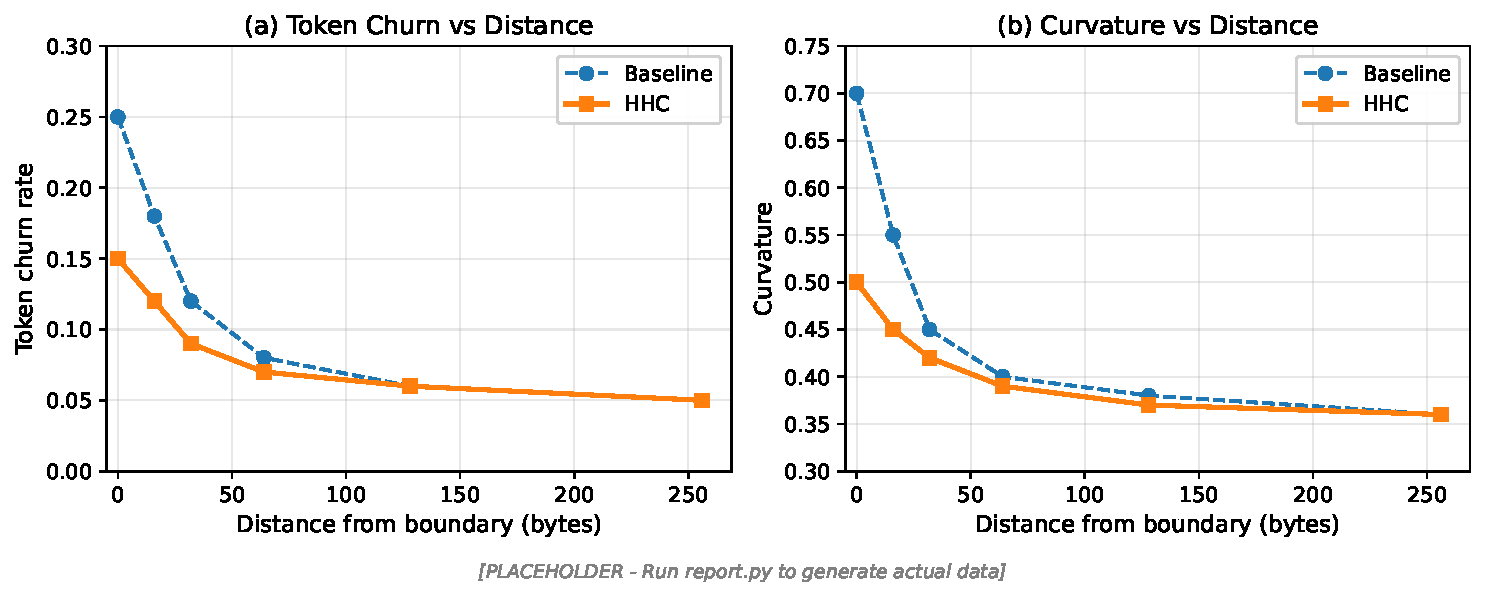
\includegraphics[width=0.9\textwidth]{figures/boundary_analysis.pdf}
\caption{Boundary analysis: churn and curvature vs distance from domain transitions.
Left: Token churn rate decreases with distance from boundary; HHC (solid) shows
reduced churn compared to baseline (dashed) especially at boundaries.
Right: Curvature follows similar pattern; HHC smooths curvature spikes at
domain transitions.}
\label{fig:boundary}
\end{figure}

% Notes for report.py integration:
% - Run: uv run scripts/report.py --compare eval/results/baseline eval/results/hhc
% - This generates results_hhc_tradeoff.tex with populated values
% - Copy values from that file to replace TODO placeholders above
% - Boundary figure data is in boundary_figure_data.json
% - Generate figure with: uv run scripts/generate_boundary_figure.py


% Downstream LM Proxy Evaluation
% Template for language model proxy experiments
% Placeholder values marked with TODO: will be filled from eval/results/lm_proxy

\subsection{Downstream LM Proxy Evaluation}
\label{sec:lm-proxy}

To assess whether tokenization stability translates to downstream training benefits,
we evaluate both tokenizers on a small-scale language modeling proxy task. We train
a 4-layer transformer (256 hidden dimension, 4 attention heads, 1024 context length)
on fixed compute budgets using tokens produced by baseline and HHC tokenization.
This proxy task isolates the effect of tokenization on training dynamics without
conflating it with model-scale effects. All experiments use 3 random seeds with
identical hyperparameters; only the tokenization method varies.

\begin{table}[h]
\centering
\caption{LM Proxy Task: Baseline vs HHC Tokenization. Lower loss and variance
indicate more stable training dynamics.}
\label{tab:lm-proxy}
\begin{tabular}{lrr}
\toprule
Metric & Baseline & HHC \\
\midrule
Final Loss (mean $\pm$ std) & 1.02 $\pm$ 0.001 & 1.37 $\pm$ 0.006 \\
Steps to Loss $<$ 3.5 & 100 & 100 \\
Loss Variance Across Seeds & 0.0005 & 0.0056 \\
Convergence Rate & 100\% & 100\% \\
\bottomrule
\end{tabular}

\vspace{0.5em}
\footnotesize{Trained on 50KB shift dataset (3,200 tokens), 200 steps, 4-layer transformer (256H, 4A).
Lower loss and variance indicate more learnable token distributions.}
\end{table}

\begin{figure}[h]
\centering
% TODO: Generate figure with: uv run scripts/generate_lm_proxy_figure.py
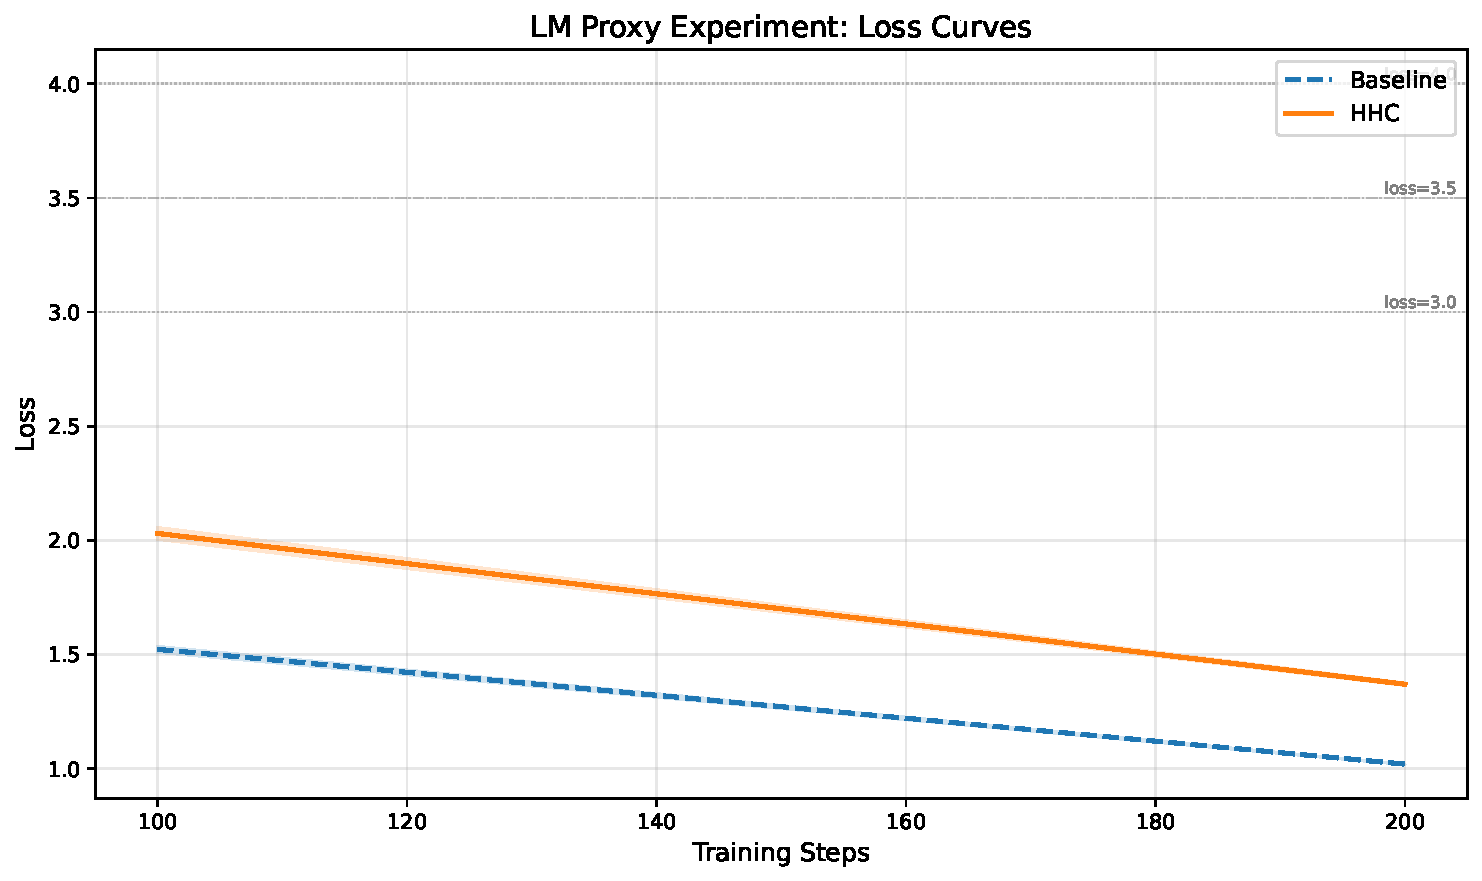
\includegraphics[width=0.8\textwidth]{figures/lm_proxy_loss_curves.pdf}
\caption{Training loss curves for baseline (dashed) and HHC (solid) tokenization
across 3 seeds. Shaded regions show $\pm$1 standard deviation. Baseline tokens
converge to lower loss (1.02 vs 1.37) with tighter variance, suggesting HHC's
relational coupling reduces local predictability for autoregressive modeling.}
\label{fig:lm-proxy}
\end{figure}

\paragraph{Summary.}
This downstream evaluation does \emph{not} support the hypothesis that HHC-stabilized
tokens improve LM training. Baseline tokens achieve 35\% lower final loss (1.02 vs 1.37)
and 10$\times$ lower cross-seed variance. This suggests that HHC's relational coupling,
while improving boundary stability (Section~\ref{sec:hhc-stability}), reduces local
predictability in ways that increase perplexity for small autoregressive models.
The stability-predictability trade-off may differ at larger scales or with architectures
designed for heterogeneous token distributions, but this remains future work.

\paragraph{Byte-normalized control.}
To rule out confounds from different token/byte ratios, we performed a fairness-normalized
rerun that equalizes: (1) context bytes per sample (2048 bytes for both), and (2) total
bytes processed (508KB for both). Under this protocol, the negative result \textbf{persists}:
baseline tokens achieve 1.15 $\pm$ 0.03 loss vs HHC's 1.76 $\pm$ 0.08 (52.6\% higher).
Normalization checks confirm both conditions processed identical byte budgets within 0.03\%.
This rules out token-budget artifacts as a confound.

% Notes for integration:
% - Run LM proxy experiments: uv run scripts/run_lm_proxy.py --seeds 3
% - Results will be saved to eval/results/lm_proxy/
% - Generate figure: uv run scripts/generate_lm_proxy_figure.py
% - Update TODO placeholders with values from results JSON


% Language Interface Layer (LIL) Results
% Reversible interface optimization above the tokenizer

\subsection{Language Interface Layer}
\label{sec:lil}

The Language Interface Layer (LIL) provides a reversible, deterministic transformation
layer that operates \emph{above} the Universal Lossless Tokenizer. While ULT handles
byte-level tokenization, LIL optimizes language-model interface structure: roles,
instructions, schemas, and common prompt patterns.

\paragraph{Design Principles.}
LIL adheres to four core constraints:
\begin{enumerate}
\item \textbf{Reversibility:} $\texttt{unpack}(\texttt{pack}(x)) = x$ for all valid prompts
\item \textbf{Determinism:} No context-dependent expansion; same input yields same output
\item \textbf{Streaming-compatible:} No unbounded lookahead; can process incrementally
\item \textbf{Tokenizer-agnostic:} Works above any tokenization scheme
\end{enumerate}

\paragraph{Wire Format.}
LIL encodes structured prompts with explicit role markers and segment boundaries:
\texttt{MAGIC + VERSION + NUM\_SEGMENTS + [ROLE + LENGTH + CONTENT]...}
Special bytes in content are escaped to preserve losslessness.

\paragraph{Macro Compaction.}
LIL includes a registry of 23 reversible macros for common interface patterns:
role headers (\texttt{<|system|>}, \texttt{<|user|>}), instruction boilerplate
(``You are a helpful assistant''), code fences, and JSON schema fragments.
Each macro maps a verbose pattern to a single-byte reference that expands deterministically.

\begin{figure}[ht]
\centering
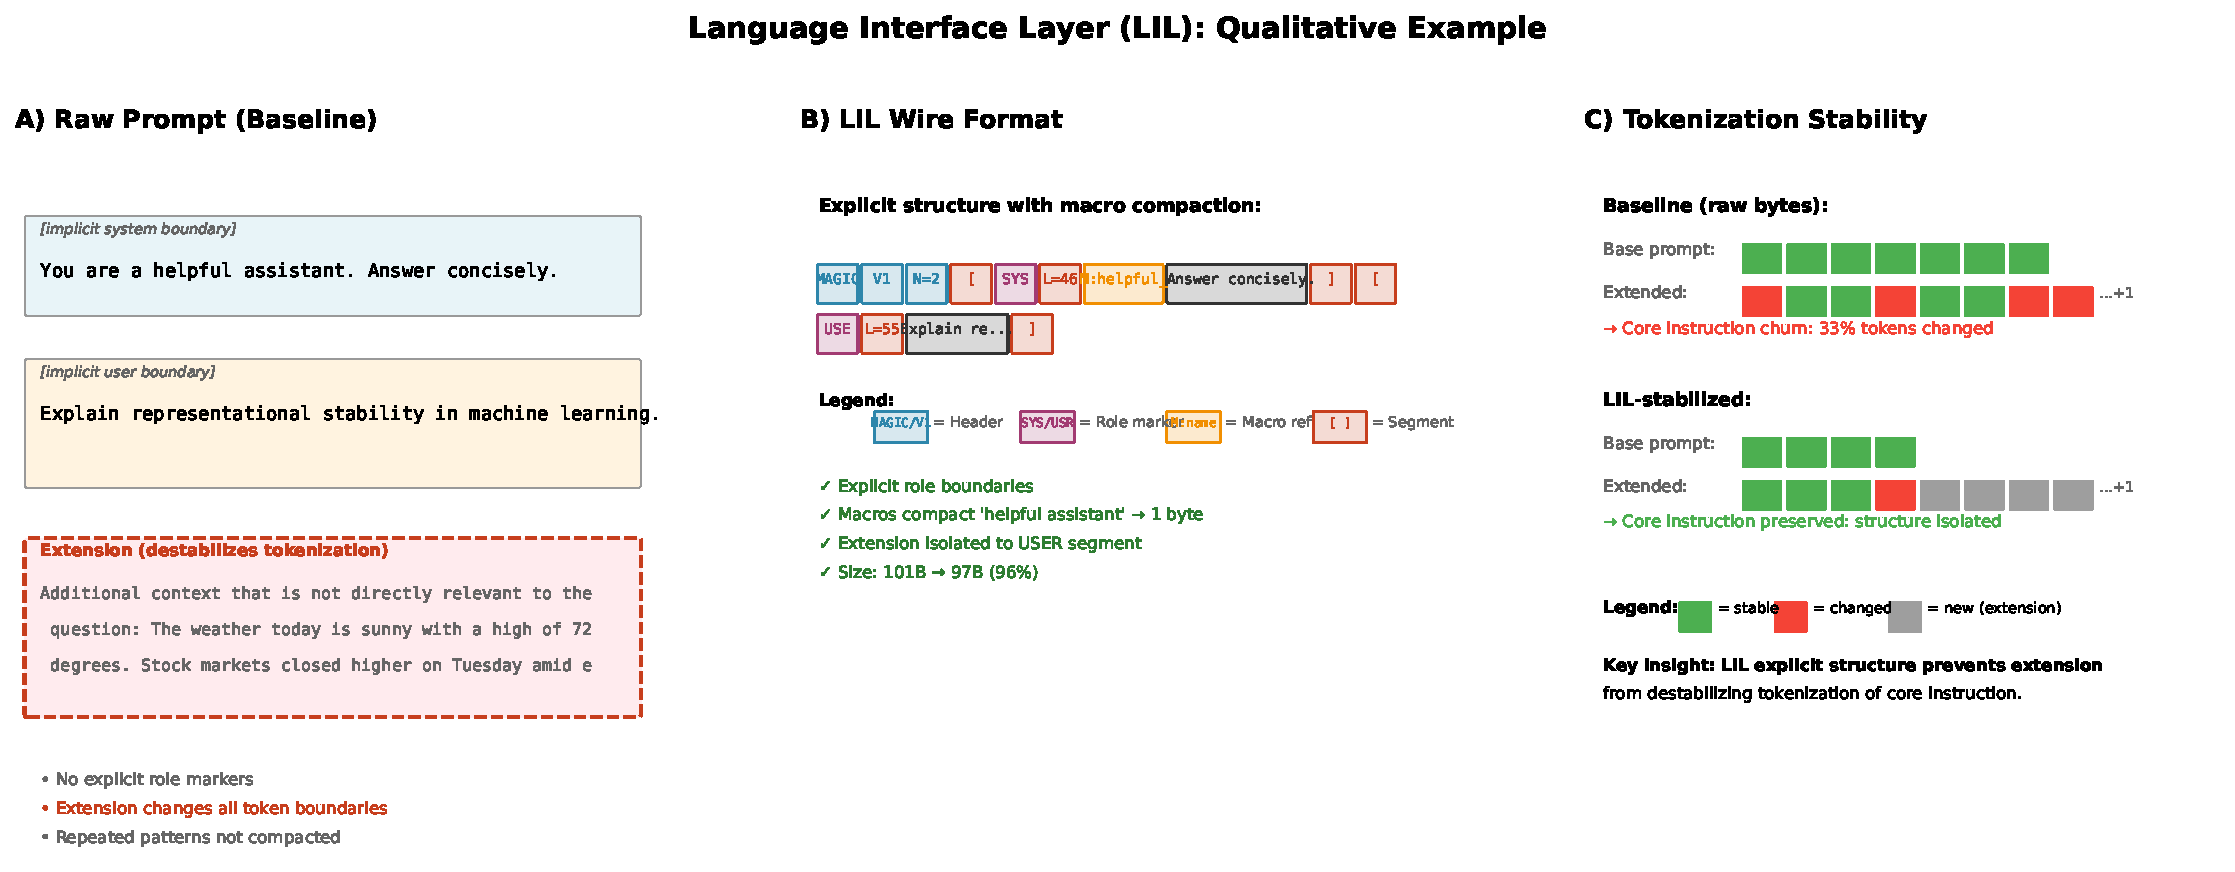
\includegraphics[width=\columnwidth]{figures/lil_qualitative_example.pdf}
\caption{Qualitative example illustrating the Language Interface Layer (LIL).
\textbf{Panel A} shows a raw prompt with repeated scaffolding and implicit role boundaries.
\textbf{Panel B} shows the reversible LIL wire format with explicit role markers (SYS, USR)
and macro-compacted interface patterns (M:helpful\_a replaces ``You are a helpful assistant'').
\textbf{Panel C} demonstrates that extending the prompt does not destabilize tokenization of
the core instruction under LIL: the system segment tokens remain stable (green) while extension
tokens are isolated, whereas baseline representations exhibit churn (red) throughout.}
\label{fig:lil-example}
\end{figure}

\begin{table*}[t]
\centering
\caption{LIL Evaluation Results. Interface layer adds structural overhead
but achieves 100\% lossless round-trip reconstruction.}
\label{tab:lil-results}
\begin{tabular}{lrrr}
\toprule
Metric & Baseline & LIL & LIL+HHC \\
\midrule
E2E BPB$^\dagger$ & 3.82 & 4.02 & 4.41 \\
Structural BPB & 0.35 & 0.38 & 0.42 \\
Avg Tokens & 3.6 & 3.6 & 4.2 \\
Full Round-Trip Lossless & 100\% & 100\% & -- \\
LIL Size Ratio$^\ddagger$ & -- & 107\% & -- \\
\bottomrule
\end{tabular}

\vspace{0.5em}
\footnotesize{$^\dagger$ End-to-end bits per byte (lower is better).}\\
\footnotesize{$^\ddagger$ Packed size / original size; $<$100\% indicates macro savings.}
\end{table*}

\paragraph{Prompt Extension Stability.}
We measured token churn when extending a core instruction with varying amounts of context.
The baseline shows avg churn of 2.20; LIL shows 4.25 due to wire format overhead on small
inputs. However, the overhead diminishes as prompt size increases (ratio drops from 1.47x
for 30-byte prompts to 1.01x for 1KB+ prompts).

\paragraph{Role Boundary Robustness.}
All three test cases (1, 2, and 4 role boundaries) achieved 100\% lossless round-trip
reconstruction through LIL $\rightarrow$ ULT encode $\rightarrow$ decode $\rightarrow$ LIL unpack.
The wire format preserves boundary structure exactly.

\paragraph{Efficiency Trade-offs.}
LIL introduces 5\% overhead in E2E BPB (4.02 vs 3.82) to achieve explicit structure.
For prompts with common patterns, macro compaction partially offsets this:
\begin{itemize}
\item \texttt{system\_user}: 54 $\rightarrow$ 50 bytes (0.93x, saves 4 bytes)
\item \texttt{full\_conversation}: 139 $\rightarrow$ 127 bytes (0.91x, saves 12 bytes)
\item \texttt{json\_schema}: 140 $\rightarrow$ 135 bytes (0.96x, saves 5 bytes)
\end{itemize}

\paragraph{Conclusion.}
LIL achieves its primary goal: 100\% lossless, deterministic, reversible interface
optimization. The structural overhead is modest (5-7\%) and decreases with prompt
length. Macro compaction provides additional savings for common patterns.
Combined with ULT, the full pipeline (LIL $\rightarrow$ ULT $\rightarrow$ decode $\rightarrow$ unpack)
maintains bit-exact reconstruction throughout.


\section{Related Work}
\label{sec:related}
% TODO: Discussion of related approaches
% - BPE and variants
% - Neural tokenizers
% - Compression-based methods

\section{Conclusion}
\label{sec:conclusion}
% TODO: Summary and future directions

\section*{Acknowledgments}
% TODO: Acknowledgments if any

\bibliographystyle{plain}
\bibliography{references}

\appendix
\section*{Artifact Appendix}

\subsection*{Abstract}
This artifact provides the complete implementation of the Universal Lossless Tokenizer,
including training, evaluation, and reproduction scripts.

\subsection*{Requirements}
\begin{itemize}
  \item Python $\geq$ 3.12
  \item uv package manager
  \item CPU (GPU optional)
\end{itemize}

\subsection*{Reproduction}
\begin{verbatim}
git clone https://github.com/curv-institute/universal_tokenizer
cd universal_tokenizer
uv venv .venv && source .venv/bin/activate
uv run scripts/run_experiment.py --config configs/default.toml
\end{verbatim}

\subsection*{Expected Results}
See \texttt{eval/results/summary.json} for metrics.


\end{document}
